\documentclass[lettersize,journal]{IEEEtran}

\usepackage{amsmath,amsfonts}
\usepackage{algorithmic}
\usepackage{algorithm}
\usepackage{array}
\usepackage[caption=false,font=normalsize,labelfont=sf,textfont=sf]{subfig}
\usepackage{textcomp}
\usepackage{url}
\usepackage{verbatim}
\usepackage{graphicx}
\usepackage{cite}

\hyphenation{op-tical net-works semi-conduc-tor IEEE-Xplore quan-ti-za-tion pho-ton-ic}

\begin{document}

\title{Quantization-Aware Differentiable Architecture Search for Photonic-Compatible Neural Networks}

\author{Filippo~Lucchesi%
\thanks{F. Lucchesi is with the Department of Information Engineering, M.Sc. Program in Artificial Intelligence and Data Engineering. Contact information will be added before submission.}%
}

\markboth{Journal Manuscript}%
{Lucchesi: Quantization-Aware Differentiable Architecture Search for Photonic-Compatible Neural Networks}

\maketitle

\begin{abstract}
Photonic neural networks offer high-throughput and low-latency execution of linear algebra, but practical accelerators impose constraints that are rarely considered during neural architecture design. In particular, the effective numerical resolution is commonly limited to approximately six bits, optical inputs are non-negative, convolutional kernels and neuron fan-in are bounded, and the cost of unnecessary transformations is amplified by conversion and calibration overheads. This article presents QA-DARTS, a quantization-aware differentiable architecture search framework that exposes candidate networks to low-precision weights and activations during the search itself. The framework is implemented on top of Neural Network Intelligence and extends its differentiable mixed operations with learned-step-size quantization for convolution, linear, and self-attention layers. The current search space contains seven always-residual stages and jointly selects dense convolution, depthwise-separable convolution, dilated depthwise-separable convolution, residual-only behavior, spatial self-attention, and learnable or parameter-free downsampling. A learned bounded residual scale and branch-specific signed or unsigned activation quantizers make the relaxed supernet consistent with the subsequently discretized model. The framework also includes precision-specific curricula for the difficult two-bit regime and a clean retraining-from-scratch protocol. The experimental design covers CIFAR-10 and a classification adaptation of the German Traffic Sign Detection Benchmark at six-, four-, and two-bit precision. Results are intentionally omitted while the updated experimental campaign is being completed.
\end{abstract}

\begin{IEEEkeywords}
Differentiable architecture search, hardware-aware neural architecture search, learned step size quantization, neural architecture search, photonic neural networks, quantization-aware training.
\end{IEEEkeywords}

\section{Introduction}
\IEEEPARstart{D}{eep} neural networks increasingly rely on accelerators to meet the latency and energy requirements of real-time inference. Photonic neural networks (PNNs) are a promising accelerator family because optical propagation naturally supports high bandwidth, parallel signal transport, and very low propagation latency. Integrated photonic circuits can implement matrix--vector multiplication through interferometric meshes, wavelength-selective weight banks, or hybrid photonic--electronic multiply--accumulate units \cite{demarinis2019survey,shen2017deep}. These properties make photonics attractive for workloads in which dense linear transformations dominate the execution time.

The same physical mechanisms that make PNNs attractive also impose non-idealities that are not represented by an ordinary floating-point neural network. Optical sources, modulators, detectors, and data converters introduce noise and restrict numerical resolution. Inputs encoded as optical intensity are non-negative. Optical fan-in is limited by power splitting, crosstalk, and component count, while large spatial kernels require additional hardware and optical routing. A network that performs well in an unconstrained software environment can therefore be expensive, inaccurate, or impossible to map to a photonic platform. Photonic-aware neural networks address part of this gap by incorporating device-level constraints into architecture and training choices \cite{paolini2022photonic}, but those choices are commonly made by hand.

Neural architecture search (NAS) offers a systematic alternative. In particular, differentiable architecture search (DARTS) replaces discrete architectural decisions with continuous mixtures and optimizes their mixing coefficients by gradient descent \cite{liu2019darts}. Its computational efficiency makes DARTS suitable for co-design problems in which many candidate networks must be evaluated. Nevertheless, a conventional DARTS search is normally conducted with full-precision weights and activations. Quantization is applied only after a candidate architecture has been selected. This ordering is problematic because quantization changes the relative quality of candidate operations: two blocks that are comparable in floating point can react very differently to clipping, rounding, and limited dynamic range.

QA-DARTS integrates quantization-aware training (QAT) directly into the relaxed supernet. Every candidate operation is evaluated with the same target precision that will be used after discretization. Network weights remain latent full-precision variables for optimization, but quantized copies are used in the forward pass; activation tensors are quantized at explicit boundaries throughout the model. Consequently, the architecture parameters are optimized using validation loss measured under low-precision computation rather than under an idealized surrogate.

The current implementation extends the original formulation substantially. Its contributions are as follows.

\begin{itemize}
\item It provides quantization-aware NNI mixed operations for convolution, linear layers, and multi-head self-attention. Convolutional weights use per-output-channel Learned Step Size Quantization (LSQ), while linear and attention projections use per-tensor LSQ.
\item It defines a seven-stage, always-residual search space that contains 13 independent decisions and 13,824 discrete architectures. In addition to standard and depthwise-separable convolutions, the space includes dilated depthwise-separable operators, zero main branches that realize residual-only blocks, quantized spatial self-attention, and two downsampling mechanisms.
\item It replaces the former hand-selected residual coefficient with a learned scale constrained to the interval $(0,2)$ and quantizes the main and residual branches separately before addition. This makes residual fusion part of the learned low-precision model.
\item It introduces precision-dependent stabilization. The two-bit CIFAR-10 search starts with a full-precision warm-up and a widened backbone, whereas the two-bit traffic-sign search follows a $6\rightarrow4\rightarrow2$-bit curriculum with quantizer-state transitions and an architecture-parameter warm-up.
\item It separates search, discretization, retraining, and evaluation. The selected architecture is reconstructed as a deterministic model and trained from random initialization, preventing inherited supernet weights from confounding the final assessment.
\end{itemize}

The remainder of the article reviews the photonic constraints and differentiable-search formulation, describes the quantization operators and updated search space, and defines the experimental protocol. The Results section is deliberately left empty until the current experiments and plots are complete.

\section{Background and Related Work}
\subsection{Photonic Neural Computing}
PNNs implement neural computations using optical signals and integrated photonic components. A coherent architecture can encode a matrix through a mesh of Mach--Zehnder interferometers, while wavelength-division multiplexed systems can assign weights to optical carriers using microring resonators or semiconductor optical amplifiers \cite{demarinis2019survey}. Hybrid designs often retain nonlinear activation, storage, and control in electronics while executing the most expensive linear operations optically. The precise system architecture changes the distribution of optical and electronic cost, but four constraints are consistently relevant to neural-network design.

First, numerical precision is limited. The effective number of bits is determined jointly by analog noise, device variability, thermal drift, optical loss, and data-converter resolution. This work considers six bits as the upper target and studies four- and two-bit operation as increasingly aggressive regimes. Second, optical intensity is non-negative, so activation paths are designed around non-negative tensors and ReLU-like nonlinearities. Signed quantities are still required for weights, normalized residual projections, and attention scores; these tensors receive explicit signed quantizers. Third, the fan-in of a photonic neuron cannot grow without bound. The classification head is therefore preceded by global average pooling and receives exactly 200 features. Fourth, experimentally practical spatial kernels are small. Every spatial convolution in the proposed backbone uses a $3\times3$ kernel or a $3\times3$ dilated kernel; pointwise projections use $1\times1$ kernels.

Photonic awareness is not equivalent to quantization alone. A model can satisfy a bit-width constraint yet use an unsuitable fan-in, negative optical input, excessive channel expansion, or an operation whose conversion cost overwhelms its arithmetic benefit. For this reason, QA-DARTS encodes structural constraints directly in the search space and applies quantization throughout every candidate path.

\subsection{Neural Architecture Search and DARTS}
NAS methods automate decisions that would otherwise require extensive manual exploration \cite{elsken2019nas}. Early approaches trained many independent architectures, which made the search prohibitively expensive for all but the largest compute budgets. Weight-sharing one-shot methods reduce that cost by embedding many candidates in a common supernet \cite{bender2018oneshot,guo2020singlepath}. DARTS goes further by expressing each discrete choice as a differentiable mixture.

Let $\mathcal{O}=\{o_1,\ldots,o_K\}$ be the candidates at one decision point and let $\boldsymbol{\alpha}\in\mathbb{R}^K$ be its architecture logits. The relaxed operation is
\begin{equation}
\bar{o}(x)=\sum_{k=1}^{K}p_k o_k(x), \qquad
p_k=\frac{\exp(\alpha_k)}{\sum_{j=1}^{K}\exp(\alpha_j)}.
\label{eq:mixedop}
\end{equation}
Network parameters $w$ and architecture parameters $\alpha$ are learned through the bilevel problem
\begin{equation}
\min_{\alpha}\;\mathcal{L}_{\mathrm{val}}(w^{\star}(\alpha),\alpha)
\quad\text{s.t.}\quad
w^{\star}(\alpha)=\arg\min_w\mathcal{L}_{\mathrm{train}}(w,\alpha).
\label{eq:bilevel}
\end{equation}
In practice, the two parameter groups are updated alternately using mini-batches from the training and validation partitions. At the end of search, each mixture is discretized with $k^{\star}=\arg\max_k\alpha_k$.

This relaxation introduces known biases. Parameter-free paths can learn faster than convolutional paths, mixed operations can exploit the simultaneous capacity of several candidates, and weakly polarized probabilities can make the final argmax unstable. QA-DARTS controls these effects structurally: a residual path is always present rather than competing as an ordinary candidate, zero operations are allowed only in two middle blocks, and architecture probabilities are recorded every epoch for later entropy and margin analysis.

\subsection{Quantization-Aware Training}
Quantization maps a continuous tensor to a finite set of representable values. A uniform signed quantizer with step size $s>0$, lower integer bound $Q_n$, and upper bound $Q_p$ can be written as
\begin{equation}
q(x;s)=s\,\mathrm{clip}\!\left(\mathrm{round}\!\left(\frac{x}{s}\right),Q_n,Q_p\right).
\label{eq:quantizer}
\end{equation}
For a $b$-bit signed weight, QA-DARTS uses $Q_n=-2^{b-1}$ and $Q_p=2^{b-1}-1$. Non-negative activations use $Q_n=0$ and $Q_p=2^b-1$. Rounding has zero derivative almost everywhere, so the backward pass uses the straight-through estimator (STE), treating the derivative through the rounding step as the identity inside the clipping range \cite{bengio2013ste,yin2019ste}.

DoReFa-Net demonstrated effective low-bit training through fixed transformations of weights and activations \cite{zhou2018dorefa}. The current framework instead uses LSQ as its active quantizer. LSQ learns $s$ jointly with the network and scales its gradient to prevent the step-size update from dominating optimization \cite{esser2020lsq}. With $N$ tensor elements, the implementation uses a scale proportional to
\begin{equation}
g_s=\frac{1}{\sqrt{NQ_p}}.
\label{eq:lsqgrad}
\end{equation}
Convolutional weight scales are initialized from the mean absolute value of each output channel, while linear and attention projection weights share one scale per tensor. Activation quantizers learn both a step size and an upper clipping parameter. This clipping parameter plays a role analogous to parameterized clipping in PACT \cite{choi2018pact}: it balances saturation error against the resolution lost when a fixed number of levels spans an unnecessarily wide interval.

\subsection{Efficient and Context-Aware Operators}
The updated search space combines operators with complementary inductive biases. A standard convolution jointly learns spatial and channel mixing. A depthwise-separable block factorizes that computation into a channel-wise $3\times3$ convolution and a $1\times1$ pointwise projection, reducing parameter and multiply--accumulate counts as in MobileNet \cite{howard2017mobilenets}. A dilated depthwise block increases the receptive field without increasing the physical kernel from $3\times3$ \cite{yu2016dilated}. Its dilation of two gives the sampling footprint of a $5\times5$ kernel while retaining nine spatial coefficients per channel.

Late stages additionally expose spatial multi-head self-attention \cite{vaswani2017attention}. The feature map is flattened to a token sequence, normalized, and processed by eight attention heads. Attention is offered only after the resolution has fallen to $8\times8$, limiting the quadratic score matrix to 64 tokens per head. All query, key, value, score, probability, context, and output paths are explicitly quantized, so attention is not an unquantized escape route within the supernet.

\section{QA-DARTS Framework}
\subsection{System Overview}
The implementation is built on the ModelSpace, LayerChoice, and DARTS components of Microsoft Neural Network Intelligence (NNI) \cite{nni}. NNI mutates ordinary mutable layers into mixed operations before one-shot training begins. QA-DARTS supplies custom mutation hooks for mutable convolution, linear, and multi-head-attention modules. Each hook constructs the corresponding quantized mixed operation, transfers the supernet weights, attaches the appropriate LSQ modules, and preserves the fixed target precision as metadata rather than exposing it as an architecture choice.

The end-to-end workflow is summarized below:
\begin{equation*}
\begin{array}{c}
\text{constrained model space}
\rightarrow\text{NNI mutation}\\[2pt]
\rightarrow\text{quantized supernet search}
\rightarrow\text{argmax export}\\[2pt]
\rightarrow\text{deterministic reconstruction}
\rightarrow\text{training from scratch}.
\end{array}
\end{equation*}
The search and deterministic models implement the same operators, quantization boundaries, residual scales, and width schedule. This correspondence is important: if the exported model differs semantically from the supernet path that won the search, final accuracy measures an implementation mismatch rather than architecture quality.

\subsection{Quantized Mixed Operations}
For convolution, the mutation hook obtains the effective sliced weight tensor associated with the current structural arguments. It applies a signed, per-output-channel LSQ quantizer and then evaluates the convolution. Grouped convolution is handled explicitly so that depthwise candidates remain valid when NNI represents their channel arguments inside a mixed operation. For linear layers, the same procedure is applied with a per-tensor LSQ scale.

The attention hook covers both the packed query/key/value projection used when all embedding dimensions match and the separate projection form used otherwise. It quantizes projection weights, input tokens, projected queries and keys, attention scores, softmax probabilities, the weighted context, and the output projection. Signed quantizers are used before and after linear projections and for scores; the softmax probability tensor uses an unsigned quantizer with a range-covering initialization. Masks are applied after score quantization so that a masked negative infinity is never rounded into a finite, attendable value.

Quantizers are registered as proper submodules before optimizer construction. This detail prevents a common implementation failure in which a learnable LSQ step size is created lazily during the first forward pass and is therefore absent from the optimizer. The code also verifies at training start that all mutable modules were replaced by the intended quantized runtime classes and that no standard mutable layer silently survived mutation.

\subsection{Quantized Spatial Self-Attention}
The attention candidate deserves an explicit formulation because a partially quantized implementation could receive an unfair advantage over convolutional candidates. Let $X\in\mathbb{R}^{N\times C}$ denote the $N=HW$ spatial tokens after an optional $1\times1$ input projection and layer normalization. For one attention head of dimension $d=C/h$, QA-DARTS computes
\begin{align}
\widehat{X} &= Q_s(X),\\
Q &= Q_s(\widehat{X}\,Q_w(W_Q)),\quad
K = Q_s(\widehat{X}\,Q_w(W_K)),\\
V &= Q_s(\widehat{X}\,Q_w(W_V)),
\label{eq:qkv}
\end{align}
where $Q_w$ is signed LSQ for weights and $Q_s$ is signed LSQ for activations. The score and probability paths are
\begin{align}
S &= Q_s\!\left(\frac{QK^{\mathsf{T}}}{\sqrt{d}}\right),\\
A &= Q_u\!\left(\mathrm{softmax}(S+M)\right),
\label{eq:attentionprob}
\end{align}
with mask $M$ and unsigned probability quantizer $Q_u$. Finally,
\begin{equation}
Y=Q_s\!\left(Q_s(AV)\,Q_w(W_O)\right).
\label{eq:attentionout}
\end{equation}
The heads are concatenated before the output projection, reshaped to NCHW format, batch-normalized, and passed through ReLU.

The ordering in (\ref{eq:attentionprob}) is important. Score quantization occurs before the mask is added. If a masked value of $-\infty$ were passed through a finite quantizer, clipping could turn it into an ordinary negative number and softmax would assign it nonzero probability. Applying the mask after quantization preserves exclusion semantics. Probability quantization occurs after softmax and optional dropout because those values occupy the bounded interval $[0,1]$ and are statistically different from the signed scores.

The implementation uses eight heads and does not search the number of heads. Searching it as a differentiable scalar inside NNI's mixed multi-head operation would change tensor partitioning and could invalidate weight sharing. Treating the complete attention module as one LayerChoice candidate makes its topology discrete at the same level as a convolutional block. It also ensures that all candidates at a stage produce exactly the same output shape, a requirement for the weighted sum in (\ref{eq:mixedop}).

Attention weights are per-tensor quantized, whereas convolutional filters are per-output-channel quantized. This choice reflects both implementation simplicity and the packed query/key/value representation used by PyTorch and NNI. Per-channel attention quantization is a possible extension, but it would require a carefully defined axis for the packed matrix and an equivalent frozen-model implementation. The present policy prioritizes exact agreement between the relaxed and exported networks.

The attention candidate includes an input projection only when input and output channels differ. When dimensions already match, the projection is the identity, preventing an unnecessary learned layer from biasing the comparison. Because L5--L7 operate at $8\times8$, the attention matrix for each image and head has only $64\times64$ entries. This restriction prevents the quadratic memory term from dominating the supernet, in which all candidates of a LayerChoice are evaluated during a differentiable forward pass.

\subsection{Always-Residual Block}
Every searchable stage is wrapped in an always-residual block. Let $o_l$ denote the selected or relaxed main operation at layer $l$, $P_l$ the identity or a $1\times1$ projection used to align channels, and $c_l$ a learned residual multiplier. The block computes
\begin{equation}
x_{l+1}=\mathrm{ReLU}\left(
Q^{+}_{l}\big(o_l(x_l)\big)+
Q^{\pm}_{l}\big(c_lP_l(x_l)\big)
\right),
\label{eq:residual}
\end{equation}
where $Q^{+}_{l}$ is an unsigned activation quantizer and $Q^{\pm}_{l}$ is signed when the projection ends in batch normalization. If $P_l$ is an identity operating on a ReLU output, the two-bit traffic-sign implementation uses the full unsigned codebook on that branch.

Rather than fixing the residual strength manually for each experiment, the current model learns
\begin{equation}
c_l=2\,\sigma(\rho_l),
\label{eq:residualscale}
\end{equation}
which constrains $c_l$ to $(0,2)$ while retaining an unconstrained parameter $\rho_l$. The default initialization $\rho_l=0$ gives $c_l=1$. The two-bit traffic-sign configuration starts at $c_l=0.75$ to preserve the stable operating point used by earlier low-bit experiments, while still permitting subsequent learning.

Separately quantizing the branches before addition is deliberate. Quantizing only the sum would let an unquantized residual bypass the target-precision constraint; quantizing the input once before both paths would force statistically different tensors to share a scale. Branch-local quantizers instead allow the learned ranges to adapt to the main and shortcut distributions.

\begin{figure*}[!t]
\centering
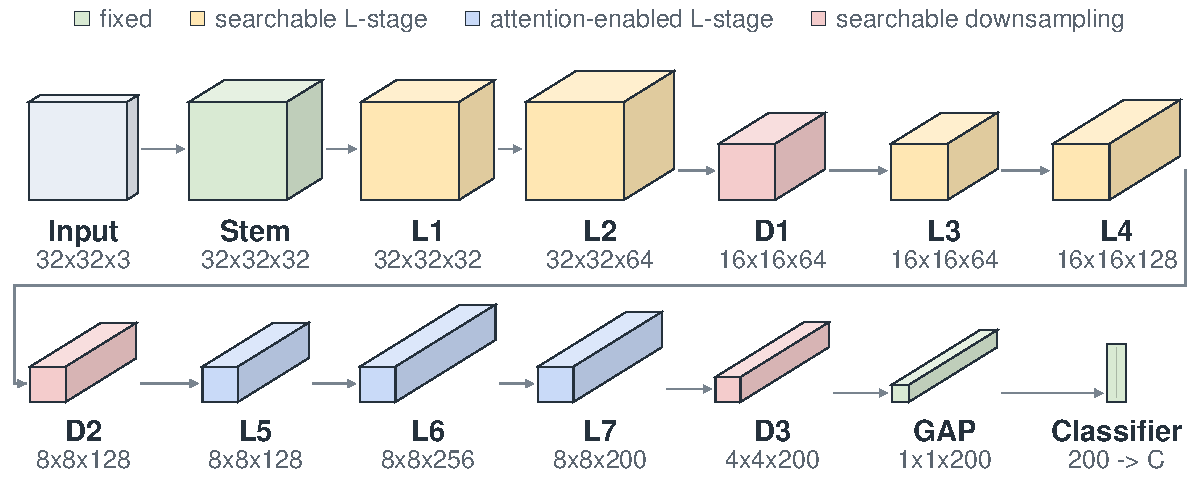
\includegraphics[width=\textwidth]{figures/qa_darts_supernet.pdf}
\caption{Topology of the current QA-DARTS supernet. Seven components are shown per row; flow proceeds across the upper row and wraps from L4 to D2 on the lower row. Block face size and stack depth encode spatial resolution and channel count, respectively, using logarithmic scaling; labels report the exact output shapes. Colors distinguish fixed components, searchable residual stages, attention-enabled stages, and downsampling decisions. L1--L7 are always-residual stages, and attention is restricted to the $8\times8$ stages.}
\label{fig:supernet}
\end{figure*}

\subsection{Current Search Space}
Table~\ref{tab:space} lists only the searchable decisions used by the current code. The quantized stem, global average pooling, and quantized classifier are fixed components shown separately in Fig.~\ref{fig:supernet}. Seven residual stages and three downsampling locations are searchable. The number of discrete architectures is
\begin{equation}
2\cdot2\cdot4\cdot4\cdot3\cdot3\cdot3\cdot2^3=13{,}824.
\label{eq:spacesize}
\end{equation}
This count excludes learned weights, LSQ parameters, and residual scales; it counts only exported structural choices.

\begin{table*}[!t]
\caption{Searchable Decisions in the Current Search Space}
\label{tab:space}
\centering
\renewcommand{\arraystretch}{1.12}
\setlength{\tabcolsep}{5pt}
\begin{tabular}{@{}>{\centering\arraybackslash}p{0.07\textwidth}>{\centering\arraybackslash}p{0.17\textwidth}>{\centering\arraybackslash}p{0.14\textwidth}>{\centering\arraybackslash}p{0.25\textwidth}>{\centering\arraybackslash}p{0.07\textwidth}@{}}
\hline
\textbf{Search decision} & \textbf{Channels} & \textbf{Input size} & \textbf{Candidate operations} & \textbf{Choices}\\
\hline
L1 & $32\rightarrow32$ & $32\times32$ & C3, DS3 & 2\\
L2 & $32\rightarrow64$ & $32\times32$ & C3, DS3 & 2\\
D1 & $64\rightarrow64$ & $32\times32$ & AP2, PC1 & 2\\
L3 & $64\rightarrow64$ & $16\times16$ & C3, DS3, Z, DDS3 & 4\\
L4 & $64\rightarrow128$ & $16\times16$ & C3, DS3, Z, DDS3 & 4\\
D2 & $128\rightarrow128$ & $16\times16$ & AP2, PC1 & 2\\
L5 & $128\rightarrow128$ & $8\times8$ & C3, DS3, A8 & 3\\
L6 & $128\rightarrow256$ & $8\times8$ & C3, DS3, A8 & 3\\
L7 & $256\rightarrow200$ & $8\times8$ & C3, DS3, A8 & 3\\
D3 & $200\rightarrow200$ & $8\times8$ & AP2, PC1 & 2\\
\hline
\end{tabular}
\vspace{3pt}

\begin{minipage}{0.78\textwidth}
\raggedright
\footnotesize
\textit{Operation legend:} C3, standard $3\times3$ convolution; DS3, depthwise $3\times3$ plus pointwise $1\times1$ convolution; DDS3, dilation-two DS3; Z, zero main branch; A8, eight-head spatial self-attention; AP2, $2\times2$ average pooling; PC1, stride-two $1\times1$ convolution with batch normalization.

\smallskip
\textit{Two-bit width note:} For the widened CIFAR-10 model, channels from the stem through L7 are $64,64,128,128,256,256,512,200$; candidates and resolutions are unchanged.
\end{minipage}
\end{table*}

The zero main branch in L3 or L4 does not remove the entire stage. It yields a residual-only block because the outer shortcut remains active, including a learned projection when channel dimensions change. Unlike a skip candidate placed directly in a DARTS mixture, the zero branch is evaluated within the same branch quantization and residual-fusion mechanism as every other option. Restricting it to two middle stages prevents the network from collapsing into a sequence of parameter-free shortcuts.

The dilated candidate expands context at a modest arithmetic cost. With dilation $d=2$ and kernel width $k=3$, the effective receptive-field width is
\begin{equation}
k_{\mathrm{eff}}=k+(k-1)(d-1)=5.
\end{equation}
The physical operation still contains nine depthwise coefficients, preserving the $3\times3$ kernel constraint. The pointwise projection then performs channel mixing.

The attention candidate is intentionally late. If a feature map has $H\times W$ positions, the score tensor has complexity $O((HW)^2C)$. At $32\times32$, this term would be 256 times larger than at $8\times8$. Restricting attention to L5--L7 makes global context available while keeping memory and search-time cost controlled. Eight heads are used in every attention candidate; the channel counts 128, 256, and 200 are all divisible by eight.

\subsection{Operation Cost and Hardware Interpretation}
For a feature map of size $H\times W$, a dense $k\times k$ convolution with $C_{\mathrm{in}}$ input channels and $C_{\mathrm{out}}$ output channels requires approximately
\begin{equation}
HWk^2C_{\mathrm{in}}C_{\mathrm{out}}
\label{eq:densemacs}
\end{equation}
multiply--accumulate operations. The depthwise-separable alternative requires
\begin{equation}
HW\left(k^2C_{\mathrm{in}}+C_{\mathrm{in}}C_{\mathrm{out}}\right).
\label{eq:dsmacs}
\end{equation}
The zero main branch adds no main-path multiplication, although its residual projection can still incur a $1\times1$ cost when channels change. These alternatives let DARTS decide where dense feature transformation is justified and where feature reuse or factorized processing is sufficient.

The search is presently accuracy-driven rather than directly multi-objective. Equations (\ref{eq:densemacs}) and (\ref{eq:dsmacs}) are therefore not added to the loss. Nevertheless, the discrete operator set exposes architectures with substantially different arithmetic, parameter, and anticipated optical resource demands. Recording these costs for every exported model enables a post-search Pareto analysis, and the same quantities can later be promoted to differentiable regularizers when hardware measurements become available.

\subsection{Discretization and Deterministic Reconstruction}
At the end of search, NNI exports the maximum-probability candidate at every LayerChoice. QA-DARTS stores semantic candidate names alongside architecture probabilities, avoiding the fragile practice of interpreting candidates solely by numeric index. The deterministic model reconstructs standard, depthwise, dilated, zero, and attention paths from the exported dictionary and retains the same width schedule, residual-scale parameterization, quantization boundaries, and downsampling choices.

All learned supernet weights are discarded for the primary evaluation. The reconstructed architecture is initialized again and optimized from scratch. This design distinguishes two questions: whether the relaxed supernet can fit the data and whether the exported discrete architecture is intrinsically trainable at the target precision. Reusing supernet weights would mix these questions and could favor operations that received more optimization during the shared-weight search.

\begin{algorithm}[!t]
\caption{QA-DARTS Search and Export}
\label{alg:qadarts}
\begin{algorithmic}[1]
\STATE Define photonic-compatible ModelSpace $\mathcal{S}$
\STATE Mutate convolution, linear, and attention modules into LSQ mixed operations
\STATE Initialize weights $w$, architecture logits $\alpha$, quantizer parameters $s$, and residual logits $\rho$
\FOR{epoch $t=0,\ldots,T-1$}
    \STATE Set active precision according to the experiment schedule
    \FOR{each training/validation mini-batch pair}
        \STATE Update $w,s,\rho$ using quantized training loss
        \IF{architecture warm-up is complete}
            \STATE Update $\alpha$ using quantized validation loss
        \ENDIF
    \ENDFOR
    \STATE Record softmax probabilities, entropy, margins, and validation metrics
\ENDFOR
\STATE Export $o_l^{\star}=\arg\max_o\alpha_{l,o}$ at every decision
\STATE Reconstruct deterministic model and reinitialize all trainable parameters
\STATE Train and evaluate the fixed architecture at the target bit width
\end{algorithmic}
\end{algorithm}

\section{Precision Management and Optimization}
\subsection{Weight and Activation Quantization Policy}
The quantization policy follows the statistics of each tensor rather than applying one rule indiscriminately. Convolutional filters use signed per-output-channel LSQ because different filters may have markedly different ranges. Linear and attention matrices use signed per-tensor LSQ. Tensors following ReLU use unsigned activation LSQ and can devote all $2^b$ codes to non-negative values. Projection residuals and normalized attention tensors use signed activation LSQ. Softmax probabilities use unsigned quantization over $[0,1]$.

The four- and two-bit activation quantizers perform a one-time data-dependent initialization on their first training batch. Given a clipped activation tensor $a$ and $Q_p=2^b-1$, the initial step is proportional to
\begin{equation}
s_0=\frac{2\,\mathbb{E}[|a|]}{\sqrt{Q_p}}.
\label{eq:actinit}
\end{equation}
Thereafter, the step and clipping bound are learned. The six-bit path starts from a fixed step and also learns it during training. For the multi-precision two-bit traffic-sign curriculum, independent LSQ states are maintained for two, four, and six bits so that returning to a precision does not overwrite another precision's calibrated range.

\subsection{Two-Bit Stabilization}
Two-bit training is qualitatively harder than four- or six-bit training: weights have only four signed codes and unsigned activations only four non-negative codes. An abrupt transition from random initialization to two-bit computation can yield noisy gradients before useful features or quantizer ranges have formed. The current code uses two stabilization strategies, selected according to the dataset.

For CIFAR-10, the two-bit supernet is widened from the baseline channel schedule $[32,32,64,64,128,128,256,200]$ to $[64,64,128,128,256,256,512,200]$. The classifier input remains 200 to preserve the fan-in constraint. Search begins with 30 full-precision epochs; architecture updates are also delayed for those 30 epochs. Training then switches directly to two-bit computation, while validation always executes the target two-bit path. The deterministic two-bit model uses a shorter staged start: 10 full-precision epochs, 20 four-bit epochs, and then the target precision.

For the smaller traffic-sign dataset, the search follows a progressive quantization schedule: 50 epochs at six bits, 50 at four bits, 30 at two bits for adaptation, and the remainder at two bits. Architecture updates are held during the first 130 epochs. At each $6\rightarrow4$ or $4\rightarrow2$ transition, LSQ weight steps are refreshed in place from the active weights, optimizer moment state is cleared, and batch-normalization running statistics are reset. The parameter objects themselves are preserved so that the optimizer continues to track the correct trainable variables. The deterministic two-bit traffic-sign model uses 50 full-precision and 50 four-bit epochs before continuing at two bits.

Validation is always performed at the final target precision, independently of the active warm-up phase. This avoids reporting optimistic validation accuracy from a higher-precision path and ensures that checkpoint selection is aligned with deployment conditions.

\subsection{Optimization and Reproducibility}
Network weights, quantizer parameters, and residual scales are optimized with stochastic gradient descent (SGD), momentum $0.9$, and cosine annealing to a minimum learning rate of $10^{-3}$. CIFAR-10 uses no weight decay in the current search code; GTSDB uses $5\times10^{-4}$. The architecture learning rate is $10^{-3}$. Gradients are clipped to a maximum norm of one, which reduces instability from the STE and from low-bit precision transitions.

The implementation fixes the Python, NumPy, and PyTorch random seeds to 42, initializes CUDA seeds when available, enables deterministic PyTorch algorithms, disables cuDNN benchmarking, and disables tensor-float-32 paths. Data-loader workers receive deterministic seeds. These settings reduce run-to-run variation, although exact reproducibility can still depend on the software stack and hardware implementation.

Architecture logits are excluded from the ordinary SGD optimizer because NNI's DARTS strategy owns their update. Runtime checks count the installed quantized mixed operations and fail if any mutable convolution, linear, or attention module bypasses the custom hooks. Alpha trajectories are captured once per epoch and logged with semantic operation labels for probability, entropy, and polarization plots.

\section{Experimental Methodology}
\subsection{Research Questions}
The updated experiments are designed to answer four questions without reusing numerical claims from the previous search space.

\begin{enumerate}
\item Can the current QA-DARTS search converge to well-polarized decisions at six, four, and two bits?
\item Which operation families are selected as precision decreases, especially dilated convolution, attention, and residual-only middle stages?
\item How much accuracy is lost between the relaxed supernet and the discretized architecture retrained from scratch?
\item What parameter, operation-count, and approximate arithmetic trade-offs arise from the discovered structures?
\end{enumerate}

The primary outcome is test accuracy of the retrained discrete architecture. Search validation accuracy is diagnostic rather than final. Secondary outcomes include search entropy, top-one probability margin, parameter count, multiply--accumulate estimates, and wall-clock time.

\subsection{Datasets and Partitions}
CIFAR-10 contains 60,000 color images of size $32\times32$ in ten balanced classes \cite{krizhevsky2009cifar}. The official 50,000-image training set is split stratifiably into 40,000 training and 10,000 validation samples. The official 10,000-image test set is held out until final evaluation. Training augmentation consists of a random $32\times32$ crop after four-pixel padding, horizontal flipping, rotation by at most $15^{\circ}$, and Cutout with a $16\times16$ mask. Validation and test images are converted to tensors without augmentation.

The German Traffic Sign Detection Benchmark (GTSDB) contains road-scene images and bounding-box annotations for traffic signs \cite{houben2013gtsdb}. The current loader converts the detection benchmark into a 43-class classification task. Every annotated sign is cropped from its source image, resized to $32\times32$, and associated with its class label. Images numbered up to 599 define the training pool; later images form the held-out test pool. Twenty percent of the training crops from each available class are assigned to validation. Training augmentation uses random rotation by at most $15^{\circ}$, brightness/contrast/saturation/hue jitter, and Cutout. Horizontal flips are not used because a flip can change traffic-sign semantics. Validation and test crops receive only resizing and tensor conversion.

The training subset updates network and quantizer parameters, while the validation subset updates architecture parameters and supports checkpoint selection. The final test set is used only after the architecture has been exported and retrained from scratch.

\subsection{Experiment Matrix}
Table~\ref{tab:protocol} records the configurations currently implemented. The six- and four-bit searches share the baseline backbone. Two-bit CIFAR-10 uses the widened channels described in Table~\ref{tab:space}; two-bit GTSDB retains the baseline widths but uses the progressive precision curriculum.

\begin{table*}[!t]
\caption{Current Search and Retraining Protocol}
\label{tab:protocol}
\centering
\renewcommand{\arraystretch}{1.13}
\begin{tabular}{|l|c|c|c|c|p{0.31\textwidth}|}
\hline
Dataset / precision & Batch & Search epochs & Weight LR & Weight decay & Stabilization and retraining schedule\\
\hline
CIFAR-10 / 6 bit & 128 & 400 & $2\times10^{-2}$ & 0 & Direct six-bit search; deterministic model retrained for 400 epochs\\
CIFAR-10 / 4 bit & 128 & 400 & $2\times10^{-2}$ & 0 & Data-calibrated activation LSQ; deterministic model retrained for 400 epochs\\
CIFAR-10 / 2 bit & 128 & 400 & $2\times10^{-2}$ & 0 & Widened backbone; 30 full-precision search warm-up epochs; scratch schedule: 10 full precision, 20 four bit, then two bit\\
GTSDB / 6 bit & 32 & 200 & $2\times10^{-2}$ & $5\times10^{-4}$ & Direct six-bit search; deterministic model budget 250 epochs\\
GTSDB / 4 bit & 32 & 200 & $2\times10^{-2}$ & $5\times10^{-4}$ & Data-calibrated activation LSQ; deterministic model budget 250 epochs\\
GTSDB / 2 bit & 32 & 400 & $5\times10^{-2}$ & $5\times10^{-4}$ & Search: 50 epochs at six bit, 50 at four bit, 30 at two-bit adaptation, then two bit; scratch: 50 full precision, 50 four bit, then two bit\\
\hline
\end{tabular}
\end{table*}

All searches use architecture learning rate $10^{-3}$, gradient clipping at one, and cosine annealing of the network learning rate to $10^{-3}$. Search-time drop path is disabled. The final deterministic model is initialized independently, trained with the exported operations, and evaluated with quantized inference.

\subsection{Architecture-Search Diagnostics}
An exported architecture alone does not reveal whether DARTS made confident decisions. For each decision $l$, the recorded softmax distribution $p_{l,k}$ is summarized by normalized entropy
\begin{equation}
\tilde{H}_l=-\frac{1}{\log K_l}\sum_{k=1}^{K_l}p_{l,k}\log p_{l,k},
\label{eq:entropy}
\end{equation}
which ranges from zero for a one-hot distribution to one for a uniform distribution. A complementary margin is
\begin{equation}
m_l=p_{l,(1)}-p_{l,(2)},
\end{equation}
where $p_{l,(1)}$ and $p_{l,(2)}$ are the largest and second-largest probabilities. Low entropy and a large margin indicate a robust argmax; high entropy or a small margin signals that the discrete choice may be sensitive to random seed or optimization noise.

The final report will plot trajectories of $p_{l,k}$, $\tilde{H}_l$, and $m_l$ for all 13 decisions. Operation names are preserved semantically, so plots will identify, for example, \emph{dilated depthwise} or \emph{attention} rather than an implementation-dependent option index.

\subsection{Final-Model Evaluation}
Each exported model will be retrained with at least the same seed and data partition used in search. Final reporting will include best validation accuracy, corresponding held-out test accuracy, parameter count, estimated multiply--accumulates, selected operation sequence, and training time. To separate architectural effects from optimization variance, repeated scratch runs should be reported with mean and standard deviation once compute permits. Confusion matrices and per-class recall are particularly relevant for GTSDB because the cropped class distribution is not balanced.

The comparison between supernet and scratch training will use curves on the same epoch axis but will not interpret supernet accuracy as deployable-model accuracy. A supernet layer evaluates a weighted sum of several candidates, whereas the exported model retains only one. The difference between the two curves therefore measures both discretization loss and the consequences of shared-weight training.

\subsection{Ablations}
Three ablations are planned to attribute gains to individual changes in the current implementation. First, the new search space will be compared with a convolution-only space that removes attention, dilation, and the zero main branch while preserving widths and quantization. Second, the learned residual scale in (\ref{eq:residualscale}) will be compared with a fixed unit scale. Third, the two-bit curricula will be compared with direct two-bit training. Each ablation must retain the same data split, target precision, optimizer, and retraining budget so that the changed component is the only systematic difference.

For attention-containing architectures, a further diagnostic will compare quantized and unquantized attention internals while keeping convolutional quantization active. This is not a deployment configuration; it tests whether any observed preference for attention is caused by its representational value or by an accidental precision bypass.

\clearpage
\section{Results}
% ---------------------------------------------------------------------------
% RESULTS RESERVATION: replace everything down to RESULTS RESERVATION END with
% the updated results, architecture tables, plots, and discussion.  This block
% deliberately reserves three full IEEE pages in the current 12-page draft.
% ---------------------------------------------------------------------------
\vspace*{\fill}
\clearpage
\mbox{}\vfill
\clearpage
\mbox{}\vfill
\clearpage
% RESULTS RESERVATION END

\section{Limitations and Future Directions}
The framework models a constrained photonic target but does not yet simulate a specific fabricated device. The six-bit ceiling, non-negative activation path, fan-in limit, and kernel restrictions are architectural proxies. Thermal drift, shot noise, component mismatch, optical loss, calibration frequency, and converter energy are not injected into the current forward model. Conclusions about physical deployment will therefore require hardware measurements or a validated device simulator.

Search cost is also not an explicit objective. The operator set contains efficient alternatives, but DARTS minimizes validation loss alone. A natural extension is multi-objective search with differentiable latency, energy, optical component count, or conversion penalties. Such costs should be calibrated on the intended platform; generic multiply--accumulate counts do not capture wavelength routing, electro-optic conversion, memory traffic, or attention-specific data movement.

The search uses one fixed precision per final model. Mixed-precision search could allocate more bits to sensitive projections and fewer bits to robust depthwise or residual paths. The multi-precision quantizer state already implemented for the two-bit curriculum provides part of the required infrastructure, but bit width would need to become a properly regularized architecture decision rather than a training-only schedule.

The evaluation is limited to two $32\times32$ image-classification tasks. Larger images and non-vision workloads may change the value of attention, dilation, and downsampling. Time-series inference, optical communications, and scientific signal processing are especially relevant future domains. Finally, physical validation on a PNN prototype is essential. It would determine whether the architecture preferences learned from quantization and structural constraints survive real optical noise and calibration behavior.

\section{Conclusion}
This article formulated QA-DARTS as an end-to-end method for searching neural architectures under photonic-compatible precision and structural constraints. The updated framework quantizes the relaxed supernet rather than applying low precision after architecture selection, and it maintains semantic equivalence between search and deterministic retraining. Its current search space combines seven always-residual stages, learned residual scaling, efficient and dilated convolutions, residual-only middle blocks, late spatial self-attention, and searchable downsampling while preserving a 200-feature classification fan-in. Precision-specific warm-up schedules address the instability of two-bit optimization without changing the target-precision validation path. The resulting methodology provides a controlled basis for evaluating which architectural patterns remain useful as numerical resolution decreases. Quantitative conclusions will be added after the updated searches, scratch retraining runs, and plots have been completed.

\section*{Acknowledgments}
The author thanks Marco Cococcioni, Nicola Andriolli, and Emilio Paolini for supervision and guidance on photonic-aware neural-network design and quantization-aware architecture search.

\begin{thebibliography}{27}

\bibitem{demarinis2019survey}
L. De Marinis, M. Cococcioni, P. Castoldi, and N. Andriolli, ``Photonic neural networks: A survey,'' \emph{IEEE Access}, vol. 7, pp. 175827--175841, 2019.

\bibitem{paolini2022photonic}
E. Paolini, L. De Marinis, M. Cococcioni, L. Valcarenghi, L. Maggiani, and N. Andriolli, ``Photonic-aware neural networks,'' \emph{Neural Computing and Applications}, 2022.

\bibitem{shen2017deep}
Y. Shen, N. C. Harris, S. Skirlo, \emph{et al.}, ``Deep learning with coherent nanophotonic circuits,'' \emph{Nature Photonics}, vol. 11, no. 7, pp. 441--446, 2017.

\bibitem{elsken2019nas}
T. Elsken, J. H. Metzen, and F. Hutter, ``Neural architecture search: A survey,'' \emph{Journal of Machine Learning Research}, vol. 20, no. 55, pp. 1--21, 2019.

\bibitem{liu2019darts}
H. Liu, K. Simonyan, and Y. Yang, ``DARTS: Differentiable architecture search,'' in \emph{Proc. Int. Conf. Learning Representations (ICLR)}, 2019.

\bibitem{nni}
Microsoft, ``Neural Network Intelligence (NNI): An open source AutoML toolkit,'' 2018. [Online]. Available: \url{https://nni.readthedocs.io/en/stable/}

\bibitem{bender2018oneshot}
G. Bender, P.-J. Kindermans, B. Zoph, V. Vasudevan, and Q. V. Le, ``Understanding and simplifying one-shot architecture search,'' in \emph{Proc. Int. Conf. Machine Learning (ICML)}, pp. 550--559, 2018.

\bibitem{guo2020singlepath}
Z. Guo, X. Zhang, H. Mu, W. Heng, Z. Liu, Y. Wei, and J. Sun, ``Single path one-shot neural architecture search with uniform sampling,'' in \emph{Proc. Eur. Conf. Computer Vision (ECCV)}, pp. 544--560, 2020.

\bibitem{zhou2018dorefa}
S. Zhou, Y. Wu, Z. Ni, X. Zhou, H. Wen, and Y. Zou, ``DoReFa-Net: Training low bitwidth convolutional neural networks with low bitwidth gradients,'' \emph{arXiv:1606.06160}, 2018.

\bibitem{esser2020lsq}
S. K. Esser, J. L. McKinstry, D. Bablani, R. Appuswamy, and D. S. Modha, ``Learned step size quantization,'' in \emph{Proc. Int. Conf. Learning Representations (ICLR)}, 2020.

\bibitem{bengio2013ste}
Y. Bengio, N. L\'eonard, and A. Courville, ``Estimating or propagating gradients through stochastic neurons for conditional computation,'' \emph{arXiv:1308.3432}, 2013.

\bibitem{yin2019ste}
P. Yin, J. Lyu, S. Zhang, S. Osher, Y. Qi, and J. Xin, ``Understanding straight-through estimator in training activation quantized neural nets,'' in \emph{Proc. Int. Conf. Learning Representations (ICLR)}, 2019.

\bibitem{choi2018pact}
J. Choi, Z. Wang, S. Venkataramani, P. I.-J. Chuang, V. Srinivasan, and K. Gopalakrishnan, ``PACT: Parameterized clipping activation for quantized neural networks,'' \emph{arXiv:1805.06085}, 2018.

\bibitem{howard2017mobilenets}
A. G. Howard, M. Zhu, B. Chen, \emph{et al.}, ``MobileNets: Efficient convolutional neural networks for mobile vision applications,'' \emph{arXiv:1704.04861}, 2017.

\bibitem{yu2016dilated}
F. Yu and V. Koltun, ``Multi-scale context aggregation by dilated convolutions,'' in \emph{Proc. Int. Conf. Learning Representations (ICLR)}, 2016.

\bibitem{vaswani2017attention}
A. Vaswani, N. Shazeer, N. Parmar, \emph{et al.}, ``Attention is all you need,'' in \emph{Advances in Neural Information Processing Systems}, vol. 30, pp. 5998--6008, 2017.

\bibitem{krizhevsky2009cifar}
A. Krizhevsky and G. Hinton, ``Learning multiple layers of features from tiny images,'' Univ. Toronto, Toronto, ON, Canada, Tech. Rep., 2009.

\bibitem{houben2013gtsdb}
S. Houben, J. Stallkamp, J. Salmen, M. Schlipsing, and C. Igel, ``Detection of traffic signs in real-world images: The German Traffic Sign Detection Benchmark,'' in \emph{Proc. Int. Joint Conf. Neural Networks (IJCNN)}, 2013.

\end{thebibliography}

\end{document}
